\section{Discussion}
\label{sec:its-discussion}

\subsection{Rasch model}
Many efforts exist to rate, rank, organize, and prioritize vulnerabilities into lists and taxonomies, such as the \gls{owasp} Top 10~\cite{wichers2017owasp}, the seven pernicious kingdoms~\cite{tsipenyuk2005seven}, the \gls{cve}~\cite{guo2009ontology,mann1999towards,baker1999development}, and the \gls{cwe}/SANS Top 25 most dangerous software errors~\cite{martin20112011}.
They are often built from the perspective of the security professional, and take into account prevalence in production, detectability by tools, and potential of impact.
These lists and taxonomies can be used as guidelines for security professionals to decide which insecurities should be prioritized.

The results from the Rasch model sometimes contradict these lists.
Injection and \gls{xxe}, for example, are typically rated high on prioritization lists because of their prevalence in production software.
According to our data, however, they are not the most difficult challenges in training.
When the developer is aware such a vulnerability is present, they are able to detect and resolve it with relative ease.
So while popular lists like \gls{owasp} Top 10 can be useful as baselines and guidelines for security teams to set their priorities, they might not be the right focus from an education perspective.
Based on the results from the Rasch model, developer training should go further than these infamous security problems and focus more on security problems involving larger pieces of code.
We can see this shift in priority in the newest draft of the \gls{owasp} Top 10\footnote{\url{https://owasp.org/Top10/}} as well.
In the new version, shown in Figure~\ref{fig:newowasptop10}, ``Injection" goes down in priority and ``\gls{xxe}" even merges with ``Security misconfiguration".
New categories are introduced such as ``insecure design", proposed as the new number 4, shifting the focus towards security flaws.

\begin{sidewaysfigure}
    \centering
    %
\begin{tikzpicture}[
    scale=0.75
    ]
    
    % SDLC blocks
    \coordinate(a1) at (10.0, 10.0);
    \coordinate(a2) at (10.3, 10.5);
    \coordinate(a3) at (10.0, 11.0);
    \coordinate(a4) at (12.8, 11.0);
    \coordinate(a5) at (13.1, 10.5);
    \coordinate(a6) at (12.8, 10.0);
    \fill[scw-yellow] (a1) -- (a2) -- (a3) -- (a4) -- (a5) -- (a6) -- cycle;
    \node[black] at (11.5,10.5) {\sffamily Plan};
    
    \coordinate(b1) at (13.0, 10.0);
    \coordinate(b2) at (13.3, 10.5);
    \coordinate(b3) at (13.0, 11.0);
    \coordinate(b4) at (15.8, 11.0);
    \coordinate(b5) at (16.1, 10.5);
    \coordinate(b6) at (15.8, 10.0);
    \fill[scw-yellow] (b1) -- (b2) -- (b3) -- (b4) -- (b5) -- (b6) -- cycle;
    \node[black] at (14.5,10.5) {\sffamily Develop};
    
    \coordinate(c1) at (16.0, 10.0);
    \coordinate(c2) at (16.3, 10.5);
    \coordinate(c3) at (16.0, 11.0);
    \coordinate(c4) at (18.8, 11.0);
    \coordinate(c5) at (19.1, 10.5);
    \coordinate(c6) at (18.8, 10.0);
    \fill[scw-yellow] (c1) -- (c2) -- (c3) -- (c4) -- (c5) -- (c6) -- cycle;
    \node[black] at (17.5,10.5) {\sffamily Build};
    
    \coordinate(d1) at (19.0, 10.0);
    \coordinate(d2) at (19.3, 10.5);
    \coordinate(d3) at (19.0, 11.0);
    \coordinate(d4) at (21.8, 11.0);
    \coordinate(d5) at (22.1, 10.5);
    \coordinate(d6) at (21.8, 10.0);
    \fill[scw-yellow] (d1) -- (d2) -- (d3) -- (d4) -- (d5) -- (d6) -- cycle;
    \node[black] at (20.5,10.5) {\sffamily Test};
    
    \coordinate(e1) at (22.0, 10.0);
    \coordinate(e2) at (22.3, 10.5);
    \coordinate(e3) at (22.0, 11.0);
    \coordinate(e4) at (24.8, 11.0);
    \coordinate(e5) at (25.1, 10.5);
    \coordinate(e6) at (24.8, 10.0);
    \fill[scw-yellow] (e1) -- (e2) -- (e3) -- (e4) -- (e5) -- (e6) -- cycle;
    \node[black] at (23.5,10.5) {\sffamily Release};
    
    % arrows -- last to first
    % 5th arrow
        %triangle
    \coordinate(i1) at (24.3, 7.2); 
    \coordinate(i2) at (24.1, 7.0); 
    \coordinate(i3) at (24.3, 6.8); 
    
    \coordinate(i4) at (24.3, 6.9); 
    \coordinate(i5) at (24.8, 6.9); 
        % top
    \coordinate(i6) at (24.8, 9.9); 
    \coordinate(i7) at (24.6, 9.9); 
    
    \coordinate(i8) at (24.6, 7.1); 
    \coordinate(i9) at (24.3, 7.1); 
    
    \node[scw-orange,left] at (24.6,9.2) {\footnotesize Breaches};
    \fill[scw-orange] (i1) -- (i2) -- (i3) -- (i4) -- (i5) -- (i6) -- (i7) -- (i8) -- (i9) -- cycle;
    
    % horizontal
    \coordinate(i10) at (24.15, 7.1); 
    \coordinate(i20) at (24.05, 7.0); 
    \coordinate(i30) at (24.15, 6.9); 
    \coordinate(i40) at (21.85, 6.9); 
    \coordinate(i50) at (21.85, 7.1); 
    \fill[scw-orange] (i10) -- (i20) -- (i30) -- (i40) -- (i50) -- cycle;
    
    
    % 4th arrow
        %triangle
    \coordinate(j1) at (21.3, 7.2); 
    \coordinate(j2) at (21.1, 7.0); 
    \coordinate(j3) at (21.3, 6.8); 
    
    \coordinate(j4) at (21.3, 6.9); 
    \coordinate(j5) at (21.8, 6.9); 
        % top
    \coordinate(j6) at (21.8, 9.9); 
    \coordinate(j7) at (21.6, 9.9); 
    
    \coordinate(j8) at (21.6, 7.1); 
    \coordinate(j9) at (21.3, 7.1); 
    
    \fill[scw-orange] (j1) -- (j2) -- (j3) -- (j4) -- (j5) -- (j6) -- (j7) -- (j8) -- (j9) -- cycle;
    % horizontal
    \node[scw-orange, left] at (21.6,9.2) {\footnotesize Code};
    \node[scw-orange, left] at (21.6,8.7) {\footnotesize analysis};
    \node[scw-orange, left] at (21.6,8) {\footnotesize Penetration};
    \node[scw-orange, left] at (21.6,7.5) {\footnotesize testing};
    
    % horizontal and back up
        %arrow ending top right
    \coordinate(i10) at (21.15, 7.1); 
    \coordinate(i20) at (21.05, 7.0); 
    \coordinate(i30) at (21.15, 6.9); 
    
    \coordinate(i40) at (13.4, 6.9); 
    \coordinate(i50) at (13.4, 9.7); 
        % top   
    \coordinate(i60) at (13.3, 9.7); 
    \coordinate(i70) at (13.5, 9.9); 
    \coordinate(i80) at (13.7, 9.7); 
    
    \coordinate(i90) at (13.6, 9.7); 
    \coordinate(i100) at (13.6, 7.1); 
    \fill[scw-orange] (i10) -- (i20) -- (i30) -- (i40) -- (i50) -- (i60) -- (i70) -- (i80) -- (i90) -- (i100) -- cycle ;
    
    \node[scw-orange, left] at (13.4,9.2) {\footnotesize Fix};
    
    
    
    
    
\end{tikzpicture}
    \includegraphics[page=23, width=\textwidth]{03-education/figures/tikzfigures.pdf}
  \caption[OWASP Top 10 2021 draft]{Some categories from the \gls{owasp} Top 10 2017 decrease in priority (marked in orange) in the new draft, other categories increase in priority (marked in blue). Three categories are merged with other categories (marked in gray). In the 2021 draft, three new categories are introduced (marked in blue).}
  \label{fig:newowasptop10} 
\end{sidewaysfigure}


We see a clear gap between knowledge and practice with these vulnerabilities being so prevalent in practice, but relatively easy to fix in training.
This is because, in a custom setting such as the \gls{scw} training platform, the developer is aware of security and able to apply their knowledge to the examples at hand.
In practice, however, the developer is focused on the functionality and other requirements of the code, and security is no longer a priority.
The cognitive burden to constantly keep track of both the functionality and the security of the code is evidently too large.
With the right processes and the right tools, this burden can be alleviated, and the prevalence of these vulnerabilities reduced.
This is the goal of Part~\ref{p:tools} of this work.

%\todo[inline]{Relate findings to some other research about the security of programming languages}

\subsection{Recommendations}
In the experiments described in the previous chapter, several algorithms were tested and adapted to learning systems.
Memory-based algorithms based on baselines have come out on top.
The best performing is the \gls{knn} baseline algorithm using the baseline-centered Pearson similarity measure.
This was expected based on the current exercise selection, as many users show a consistent bias in their ratings.
Model-based algorithms based on dimensionality reduction through matrix factorization, are often the best performing algorithms.
However, the advantages of these algorithms are often not applicable to our current data set.

\paragraph{Data sparsity}
In many recommender systems, the user-item rating matrix is rather sparse.
In Netflix, for example, few users will have watched even half the catalogue of movies.
This is also the case for the \gls{scw} training platform, especially for the largest frameworks that offer over a thousand challenges and by adapting the algorithms to learning systems, the sparsity of the data has even been increased artificially.
This data sparsity can cause some problems for \gls{cf} algorithms.

The \emph{cold start problem} occurs when a new user or item enters the system.
Because there is no item available about this user or item, it is difficult to find neighbouring items.
Matrix factorization techniques reduce the dimensions of the matrix to alleviate this problem.
In our data set only users have been included that completed a sufficient amount of challenges so that their ability level could be estimated, so this problem has been avoided.
In practice, it will still be necessary to calibrate the ability level of new users before accurate recommendations can be made.
One problem to avoid the cold start problem can then be to use a short entry test, in the form of \gls{cat}.
A procedure like this is present in other learning systems, such as Duolingo.

For new items, a trade-off needs to be made between exploitation and exploration.
In the exploitation phase the predictions from the algorithms are used to provide a recommendation to the user.
In the exploration phase, an item is recommended for which there is insufficient data, risking a bad recommendation in order to gather new information about this item.

\paragraph{Scalability}
When the number of users and items is excessively large, computing the similarity between every two users becomes an expensive procedure.
Model-based algorithms often scale better with large data sets because matrix factorization techniques are used for dimensionality reduction.
While there are many users on the \gls{scw} training platform, and the number of users is only expected to grow, in practice the data sets are split per framework.
They are not nearly large enough for scalability to be a problem, as similarity matrices for the \gls{knn} algorithms are computed in less than a minute.
These matrices only need to be computed once in a while, for example once or twice a day.

\paragraph{Synonyms}
Synonyms occur when a number of identical or very similar items have different names or entries in the data set.
Model-based techniques are capable of dealing with the synonym problem because they do not use the item names directly, but instead look for latent factors related to the items.
In our data set we do not expect many natural synonyms to exist.
While there are duplicate exercises, in the sense that they are in the same framework and about the same vulnerability type, in reality they are in different codebases, and of varying complexity.

With the learning adaptation, however, we have intentionally introduced synonyms by splitting items into separate entities based on the ability level of the users answering them.
The fact that we still see significant improvements in the model-based algorithms, who are supposed to factor out item names, is proof that these items demonstrate significantly different characteristics in the latent factor space.
This validates the hypothesis that user ability is an important factor for the recommendation of items in a learning system.
It is possible that user ability is represented in the latent factor space in one way or another.

\paragraph{Shilling attacks}
In some recommendation systems (such as for example the Amazon web store) users can be compelled to give positive recommendations towards their own material and negative recommendations towards their competitors.
While there is less incentive to do this type of intentional rating on the \gls{scw} training platform, similar scenarios have been detected.
Users in one company made it a competition to see who could gather the most points, and they created bots for this purpose.
The bots would randomly guess at first, and keep track of the correct answer for future attempts.
This resulted in several users who answered all exercises in a single framework several times over, causing worse ratings for those items as these users did not learn anything new according to the \gls{irt} estimates.
This has now been discouraged by preventing the same user from earning points through an exercise they have already solved in the past.
For the experiments of this work, data generated by these bots has been filtered out.

\paragraph{Implicit data}
Implicit data has been briefly introduced in the explanation of the SVD++ algorithm.
This algorithm not only characterizes users based on their ratings, but also based on which items they have rated.
Using implicit data like this is expected to have a big impact on prediction accuracy for systems where the user can choose items themselves.
In Netflix, for example, it can become apparent that a user constantly avoids watching movies of a certain genre, or that star a certain actor.
On the \gls{scw} platform we also see an improvement, most likely because this allows the algorithm to better distinguish between users who follow the recommended courses, and those who do not.

\subsection{Adaptation}
The proposed adaptations to learning systems in this work is not specific to software security and could be applied to other domains.
The adaptation based on processing of the data is especially easy to implement and can be applied to any \gls{cf} algorithm.
The biggest requirement is that sufficient data needs to be available to overcome problems caused by data scarcity which can be exaggerated by splitting the data even more.
In learning systems more so than in movie or music recommendations, we can expect users to rate a significant portion of the items, which makes this requirement more likely to be met.

The adaptation was less effective in model-based \gls{cf} algorithms.
One possible explanation is that the latent factors from the dimensionality reduction techniques already represented an ability estimate.
However, estimating this through the ratings alone is likely less accurate, which is why adding it more explicitly as a filter still improved the accuracy of the predictions.
It is possible to imagine a similar adaptation in other contexts where the latent factors might be doing a good job already, but small improvements can be made by computing an important factor explicitly.

%https://reader.elsevier.com/reader/sd/pii/S0950705109000161?token=5D449CD4740BAB0E3B98D60E31098B45CF1D75C3D69F058A1C397FA12A8BEB33E63692FE48A440A3190C8AE1739E8288&originRegion=eu-west-1&originCreation=20210930091431
%https://reader.elsevier.com/reader/sd/pii/S036013150400034X?token=E19FAC8FDAF7E1644408308AD34BC37A0A8657BEE89213ACC3400CB78EF55F59EC4DF5626C77FF12D4BE4262FDD3D103&originRegion=eu-west-1&originCreation=20210930092126
%https://citeseerx.ist.psu.edu/viewdoc/download?doi=10.1.1.661.3840&rep=rep1&type=pdf
%https://www.sciencedirect.com/science/article/pii/S036013150400034X
%https://www.pluralsight.com/content/dam/pluralsight2/product/iris/AdaptiveAssessments_af_v1.pdf
%https://repository.uel.ac.uk/download/e3b705a3e6417837ad1377af2f0fe65ee01cf91ecec3bda7a2a5257fca3d9808/129643/2011_Yarandi_etal_Item_Response_Theory.pdf